% Tento soubor nahraďte vlastním souborem s přílohami (nadpisy níže jsou pouze pro příklad)



\chapter{Obrázky s vygenerovanou mapou}
\begin{figure}[H]
	\centering
	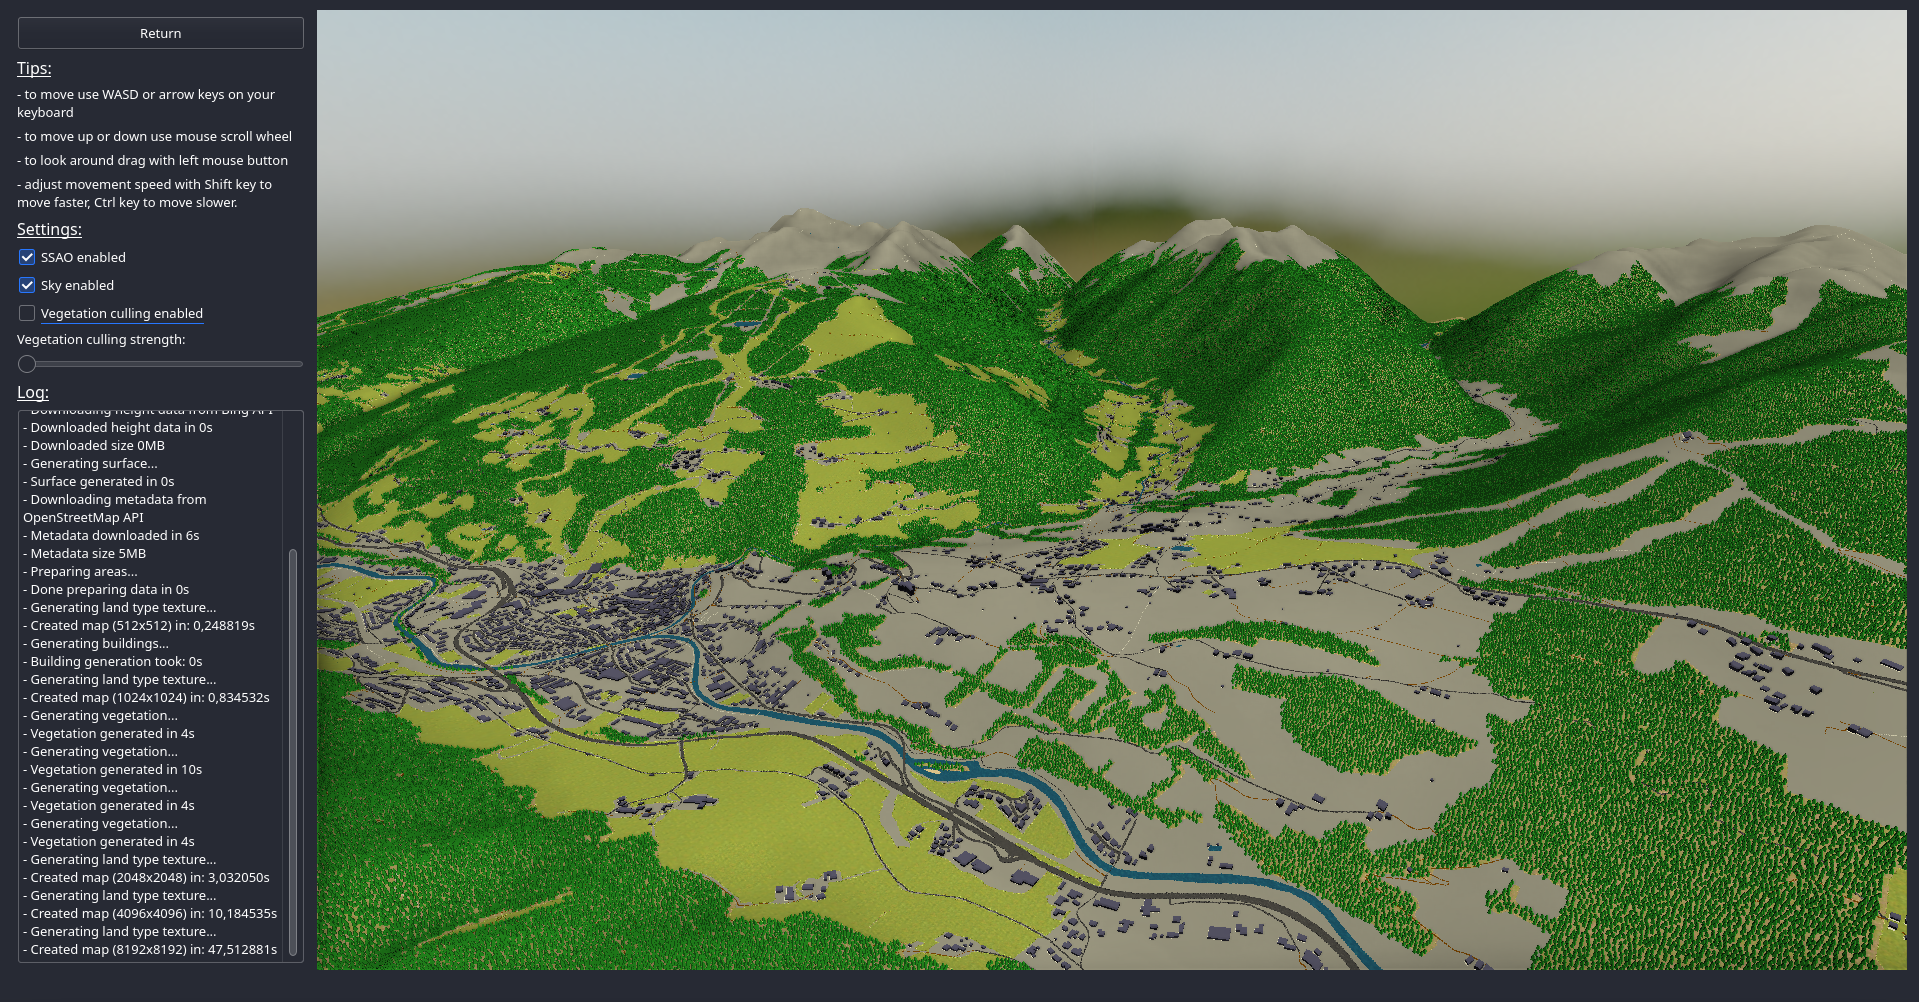
\includegraphics[width=40em]{images/results/schladming.png}
	\caption[caption]{Hornatá oblast v Rakousku okolo města Schladming.} 
	\label{img-austria}
\end{figure}

\begin{figure}[H]
	\centering
	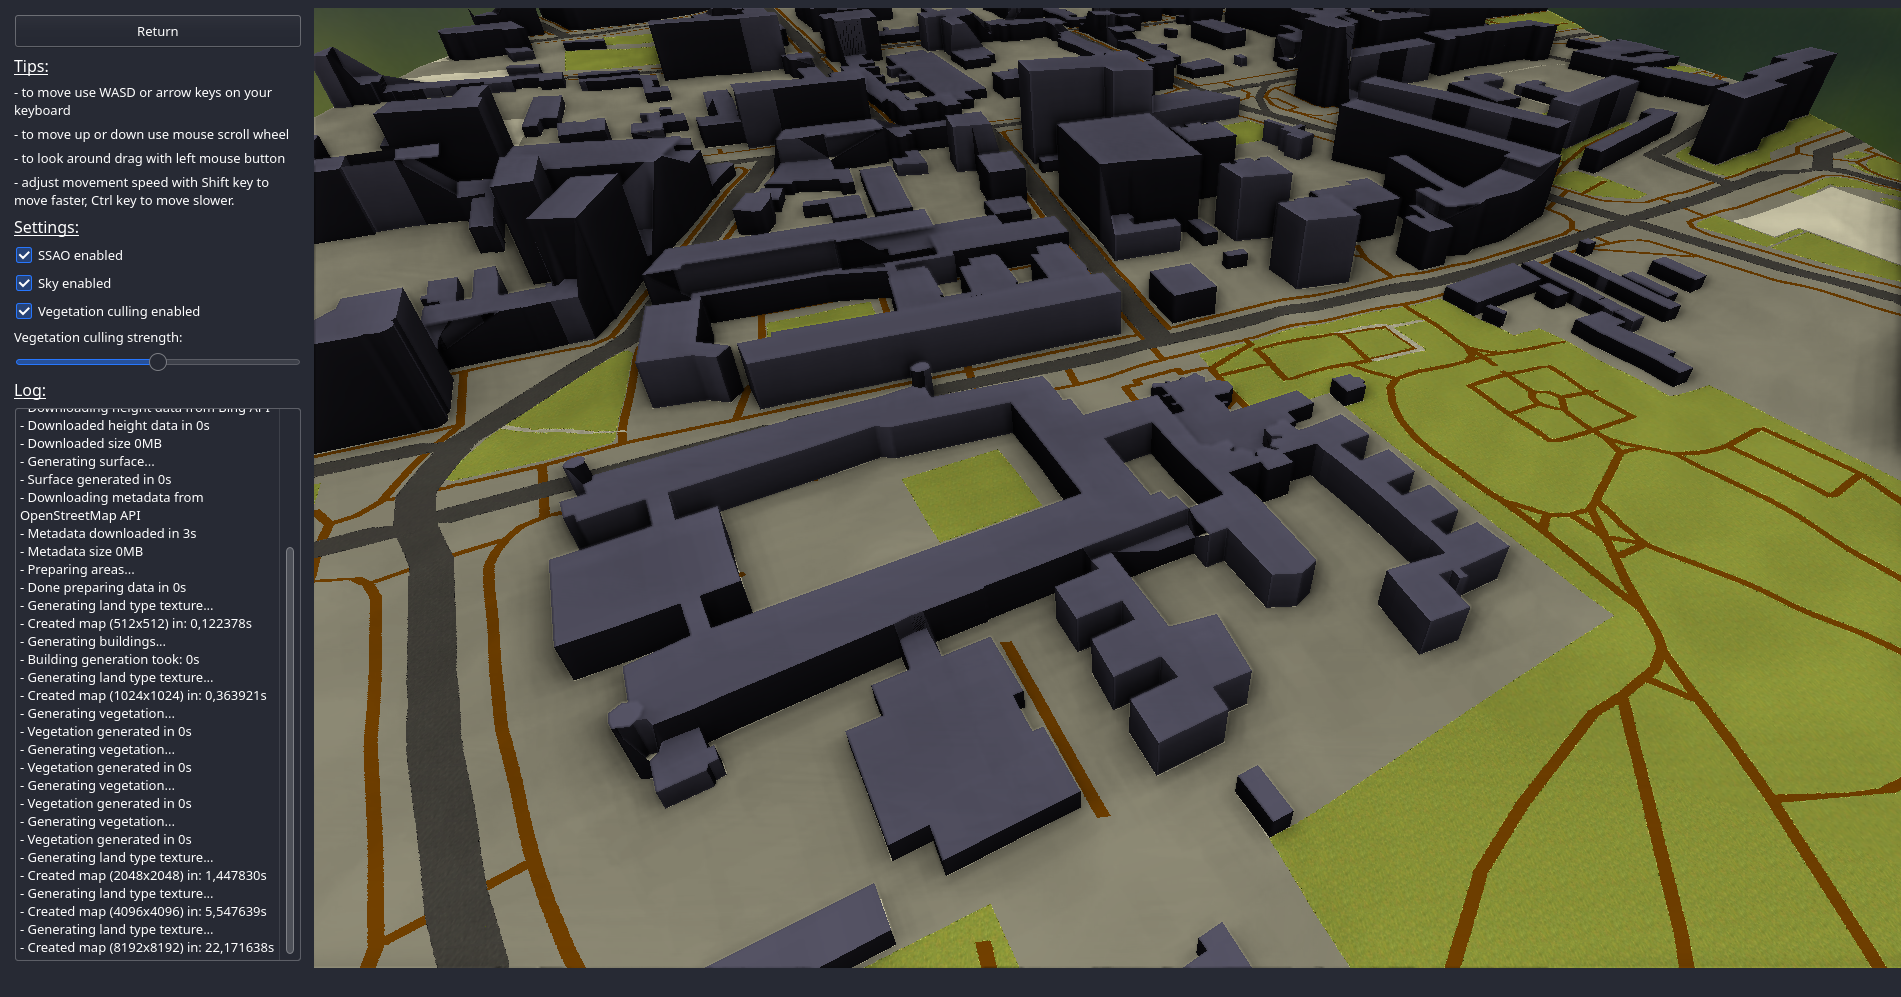
\includegraphics[width=39em]{images/results/faculty.png}
	\caption[caption]{Přiblížený pohled na VUT FIT ze západu.} 
	\label{img-fit}
\end{figure}


\begin{figure}[H]
	\centering
	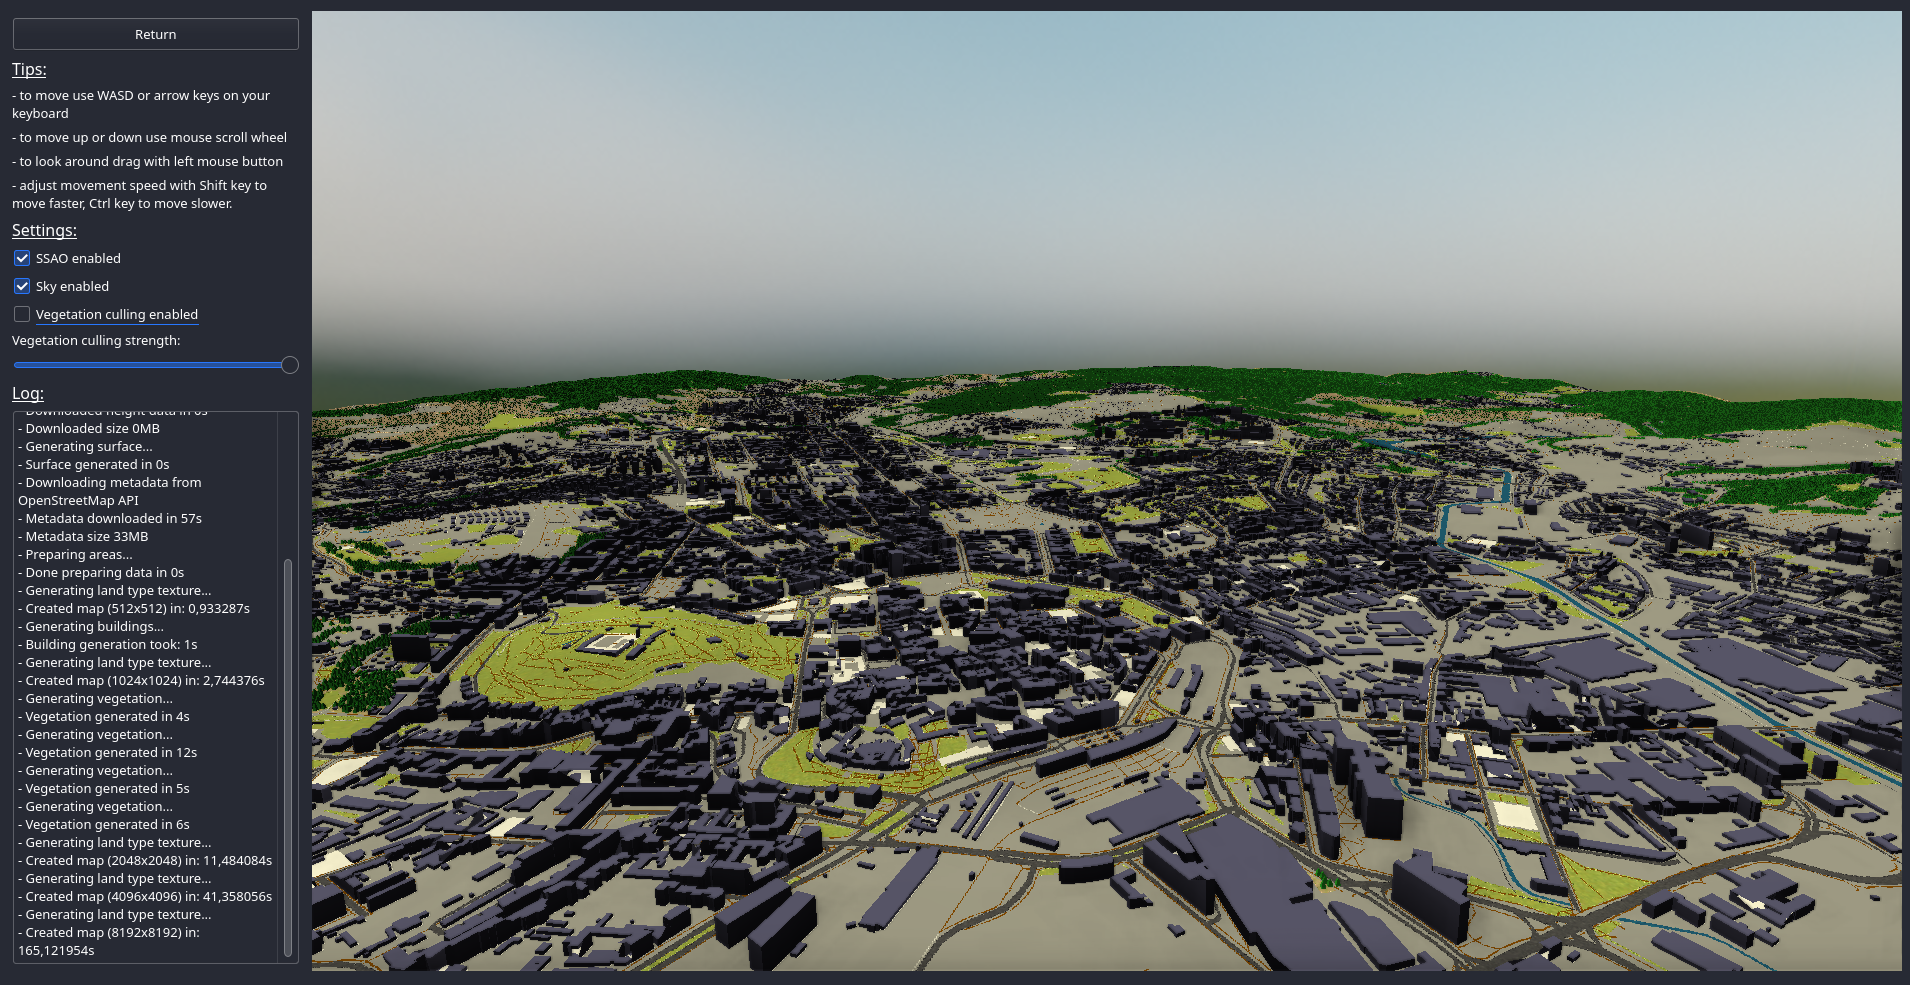
\includegraphics[width=39em]{images/results/brno.png}
	\caption[caption]{Pohled na centrum města Brna a dále na sever.} 
	\label{img-brno}
\end{figure}


\chapter{Konfigurační soubor}
Konfigurační soubor musí být aplikaci při spuštění přiřazen přes argument v příkazové řádce. Jeho formát je následující:
\begin{lstlisting}
{
  "keys":[
      {
        "service": "<name>",
        "key": "<value>"
      }
    ], "options":{
    "terrainResolution": <number>,
    "minTextureResolution": <number>,
    "maxTextureResolution": <number>,
    "textureResolutionStep": <number>,
    "generateVegetationAt": <number>,
    "randomSeed": <number>
  }

}

\end{lstlisting}
\begin{itemize}
    \item \textbf{keys} -- seznamů klíčů k autorizace na různé API
    \begin{itemize}
        \item \textbf{service} -- název služby, ke které patří klíč
        \item \textbf{key} -- hodnota klíče
    \end{itemize}
    \item \textbf{options} -- nastavení generátoru mapy
    \begin{itemize}
         \item \textbf{terrainResolution} -- rozlišení generovaného povrchu
    \item \textbf{minTextureResolution} -- minimální rozlišení textury s metadaty pro oblast
    \item \textbf{maxTextureResolution} -- maximální rozlišení textury s metadaty pro oblast
    \item \textbf{textureResolutionStep} -- násobič o kolik se změní každé další generování textury
    \item \textbf{generateVegetationAt} -- hodnota rozlišení textury s metadaty, při které bude vygenerována vegetace
    \item \textbf{randomSeed} -- vstup pro náhodné generátory čísel
    \end{itemize}
\end{itemize}


\chapter{Obsah paměťového média}

Paměťové médium ve formě CD má následující strukturu:

\begin{itemize}
    \item \textbf{src/} -- složka, obsahující veškeré zdrojové soubory práce
    \item \textbf{bin/} -- sestavené binární soubory pro systém Manjaro Linux
    \item \textbf{text/} -- zdrojové soubory k textové části práce
    \item \textbf{CMakeLists.txt} -- soubor, sloužící k překladu projektu pomocí programu cmake
    \item \textbf{Makefile} -- soubor, který využívá program make k tomu, aby vytvořil všechny potřebané složky a pomocí volání cmake sestavil celou aplikaci
    \item \textbf{config.json} -- ukázkový konfigurační souboru aplikace.
    \item \textbf{video.mp4} -- výsledek práce v podobě videa
    \item \textbf{thesis.pdf} -- tento text práce v zkompilovaném digitálním formátu
    \item \textbf{doc.pdf} -- návod ke kompilaci a použití projektu
\end{itemize}